% vim: set expandtab tabstop=4 shiftwidth=4 textwidth=80:

\documentclass{article}
\usepackage[inner=2.5cm,outer=2.5cm,bottom=1.8cm,top=1.8cm]{geometry}
\usepackage{graphicx}% Include figure files
\graphicspath{ {./graphics/} }
%\usepackage{dcolumn} % Align table columns on decimal point
%\usepackage{bm} % bold math
\usepackage{amssymb, amsmath}
\usepackage[mathscr]{euscript}

\title{Improving Product Search with Session Re-Rank\\
    \large{a Walmart data mining project}}
\author{Charles Celerier (cceleri), Bill Chickering (bchick),
        and Jamie Irvine (jirvine)}


\begin{document}

\maketitle

Walmart.com maintains an online catalog of over 2M products. Consequently,
enabling users to quickly find products that conform to their specific needs and
tastes is especially challenging. Given the difficulty of its task,
Walmart.com's product search engine does an impressive job in interpretting the
user-provided query and rapidly returning relevant results. Yet, there remains
highly significant information that is not fully leveraged. The details of a
user's online shopping session are indicative of a user's intent and
compliment---indeed, provide context for---the user-provided query. In this report
we describe and analyze a ranking scheme we call {\em Session Re-Rank} that can
potentially induce a large increase in both click-through-rates and conversions
on the first page of query results.

\section{The Technique}

{\em Session Re-Rank} works by comparing previously clicked items with the top
$N$ items returned by the search engine in reponse to a query. Items to be shown
that are sufficiently similar to previously clicked items are promoted. The
extent (i.e. number of positions) of the promotion for a particular item is a
function of its similarity to previously clicked items, its original position,
and the promotions of other items.

The similarity between an item to be shown and a previously clicked item is
determined within five distinct vector spaces: {\em click-space}, {\em
cart-space}, {\em query-space}, {\em title-space}, {\em item-space}. The
non-unique representation of an item within each of these spaces may be thought
of as a binary vector or a set of objects. (MapReduce jobs process historic
query data to construct indexes whose keys are itemids and values are lists of
the appropriate objects. Great care went into ensuring that index entries can be
accessed in $\mathcal{O}(1)$ and that two entries can be merged to compute their
intersection or union in linear time.) The similarity $J_s(A, B)$ of two items,
$A$ and $B$, within a particular space $s$ is determined using Jaccard
similarity. Similarities within particular spaces are then weighted and summed
to determine the composite similarity
\begin{equation*}
    S(A, B) = \sum_s{C_s(J_s(A, B))^{\alpha_s}},
\end{equation*}
where $C_s$ and $\alpha_s$ are tuning parameters. The score $\sigma$ attributed
to an item to be shown is then the summation of composite similarities between
itself and all previously clicked items plus the click-through-rate (CTR)
$\Gamma_i$ of the item's original position $i$
\begin{equation*}
    \sigma = \sum_{B \in P}{S(A, B)} + \Gamma_i,
\end{equation*}

where $P$ is the set of previously clicked items. 

\section{Similarity Spaces}

The premise behind {\em click-space} is that two items are similar if they are
both clicked within the same online shopping session. The dimensions, or
objects, of this space are therefore past user-sessions. The {\em clicks-index}
for the data presented in this report was contructed using approximately half of
the Walmart provided data, or about 60M queries (about 120M page views).

{\em Cart-space} is based on the notion that two items are similar is they ever
appear in a shopping cart together. The objects of this space are therefore
shopping carts. The {\em clicks-index} for the data presented in this report was
contructed using approximately half of the Walmart provided data.

Items are also considered similar if they appear in a query together. The
objects of {\em query-space} are therefore queries. We make a distinction,
however, between {\em user-queries} and {\em unique-queries}. The former are the
well-defined entities within the raw Walmart data. The latter is an abstraction
based on the notion that multiple {\em user-queries} can correspond to a single
{\em unique-query}. To derive {\em unique-queries} from our data, we cluster
{\em user-queries} as follows: two {\em user-queries} with the same search
attributes (e.g. category or price filters) are considered the same {\em
unique-query} if the strings constructed by concatenating the space-seperated,
stemmed (we use the Python stemming.porter2 module), forced to lower-case terms
from each of their rawqueries are equal. We point out that while we achieved
better results with this policy compared to simply using {\em user-queries}, we
have no reason to believe that this is the ideal way to cluster queries for use
within {\em Session Re-Rank}. Indeed, we believe one way to improve {\em Session
Re-Rank} is to optimize the query clustering policy.

{\em Title-space} is straightfoward: each item is associated with a set of terms
from its title. We ignore case, but at present do not stem, discard stop words,
or weight terms in any way. 

Finally, the structure of {\em item-space} is unique because it involves a level
of indirection. The premise here is that if items A and B are clicked in a
single user-session and items A and C are clicked in another user-session, that
items B and C are similar because they have item A in common. In this way, a
large number of relationships between items is created. {\em Item-space}
resembles {\em click-space} in that if two items are clicked during a single
session, they will have nonzero similarity. It differs from {\em click-space} in
two key respects, however. First, items that have historically never been
clicked in the same session can have nonzero similarity if they were each
clicked with a common third item. Second, if items are clicked together in many
sessions this will increase their Jaccard similarity in {\em click-space} but
not in {\em item-space}.

\section{The Data}

Walmart.com has generously supplied us with a large dataset consisting of about
250M pageviews comprising about 120M query results which occurred over about 30
days. The data includes the user-provided rawqueries together with search
attributes, visitorIds and sessionIds, shown items, clicked items, which items
were placed in a shopping cart, and which items were ultimately purchased. In
addition, they have provided detailed item information including title,
description, category, and other details. The query data was randomized with
respect to search time and then segregated into three disjoint sets. The first
set, which consists of about half of the data, was re-structured into indexes
that form four of the similarity spaces ({\em click-space}, {\em cart-space}, 
{\em query-space}, and {\em item-space}) we use to identify relationships between 
items in realtime (the remaining similarity space, {\em title-space}, was compiled
separately using the provided item data). The second set, which consists of less 
than 5\% of the data, was used for testing and optimization allowing us to refine 
our technique and tune its parameters. And the third set, which includes about 
10\% of the data, was used in the experiments described and analyzed in this 
report.

\section{The Technique vs The Experiment}

An important distinction should be made between the {\em Session Re-Rank}
technique and the experiment described in this report. Both the technique and
the experiment leverage the provided data---however, the experiment is
a simulation and a limited one at that. A key limitation is that the provided
query data is confined to what the user was actually shown. That is, the search
engine may have identified several pages worth of results in response to a {\em
user-query}, but our dataset consists only of those pages actually seen by the user.
Meanwhile, the concept behind the {\em Session Re-Rank} technique calls for a
search engine to deliver to the algorithm the top $N$ items in response to a
{\em user-query} {\em independent of the number of items ultimately shown to the
user}. As a consequence, it is difficult, if not impossible, to simulate our technique using shown
query results that are truncated because a user only viewed one or two pages. 
Even more generally, the use of historic data to demonstrate the consequences of a 
online ranking algorithm is intrinsically limited by the fact that one cannot be certain 
how users would have behaved if presented with different results. Nonetheless, 
we have done our best to conduct the most fair and informative experiment and 
analysis.

\section{The Experiment}

The goal for the experiment is to simulate {\em Session Re-Rank} using the
provided historical query data, which is limited to what users were actually
shown. Since an online implementation of our technique would receive the top $N$
items from the search engine for re-ranking prior to showing any results to a
user, the final ranking would be independent of the total number of items
actually shown (e.g. the number of page views requested by a user). Our test 
set $\chi$ therefore consists solely of queries where either all items in the
query resultset or at least $N=100$ were shown to the user. For example, if
the search engine found only 13 items in response to a query, all of these
items were shown to the user on a single page. In this case, we have the
complete query resultset and can therefore determine how {\em Session Re-Rank}
would have reordered the shown items. At the same time, if more than $N=100$
were shown to the user, we can determine the reordering regardless of whether
the query resultset is truncated since {\em Session Re-Rank} only considers
and re-ranks the first $N=100$ items.

To construct $\chi$ we therefore must discard all queries with a number of
shown results less than $N=100$ that are also divisible by 16. The reason for 
this is that Walmart.com provides two options for the number of items shown per
page: 16 or 32. Thus, by performing the experiment on this subset of the data we
precluded queries where the top $N$ items are not available to our algorithm.
The choice of $N=100$, meanwhile, is somewhat arbitrary and was made by balancing our desire
for a large test set with our desire to use a value comparable to what would be
appropriate for an online implementation. It is therefore quite possible that a
larger value of $N$ (e.g. 1000) would achieve better results in the actual
online scenario.

While we must constrain $\chi$ in this way given the nature of the available 
data, we stress that this subset is certainly biased with respect to queries 
in general. For starters, queries with short resultsets are more likely to 
have all of their resultset seen by a user, and therefore, are more likely to 
be included in $\chi$. It is not clear, however, if this particular bias
tends to under- or overestimate the effectiveness of {\em Session Re-Rank}
since, as we will show, it is more effective on longer query results. Similarly,
highly qualified queries---e.g. through the use of category or price filters---tend
to have shorter resultset, and hence, are more likely to be included in $\chi$.

% TODO: Need to comment on small differences in CTR vs position between $\chi$
% and queries in general (e.g. CTR@1 is significantly higher in $\chi$).
Just as interesting are the ways in which the queries and resultsets of $\chi$
are not biased. In Fig. \ref{fig:ctr_vs_position} we show click-through-rate (CTR)
as a function of position of the original data (i.e. not re-ranked) for both
$\chi$ and query results in general. As can be seen from the data, the quantity
and distribution of clicks within $\chi$ are essentially representative of those
in general.

\section{Metrics}

We evaluate the effectiveness of {\em Session Re-Rank} using three metrics: the 
clicks position score $\mathscr{S}$, first page CTR $\mathscr{C}$, and first page 
purchase rate $\mathscr{P}$. The clicks position score is defined
as
\begin{equation*}
    \mathscr{S} = \frac{1}{\left\vert{Q}\right\vert}\sum_{q \in Q}\sum_{c \in C_q}\Gamma_c,
\end{equation*}

where $Q$ is the test set of queries with results, $C_q$ is the set of clicks 
within the resultset of query $q \in Q$, and $\Gamma_c$ is the CTR of the position 
where click $c \in C$ occurred.

\section{Results}

\begin{figure}[htbp!]
\centering
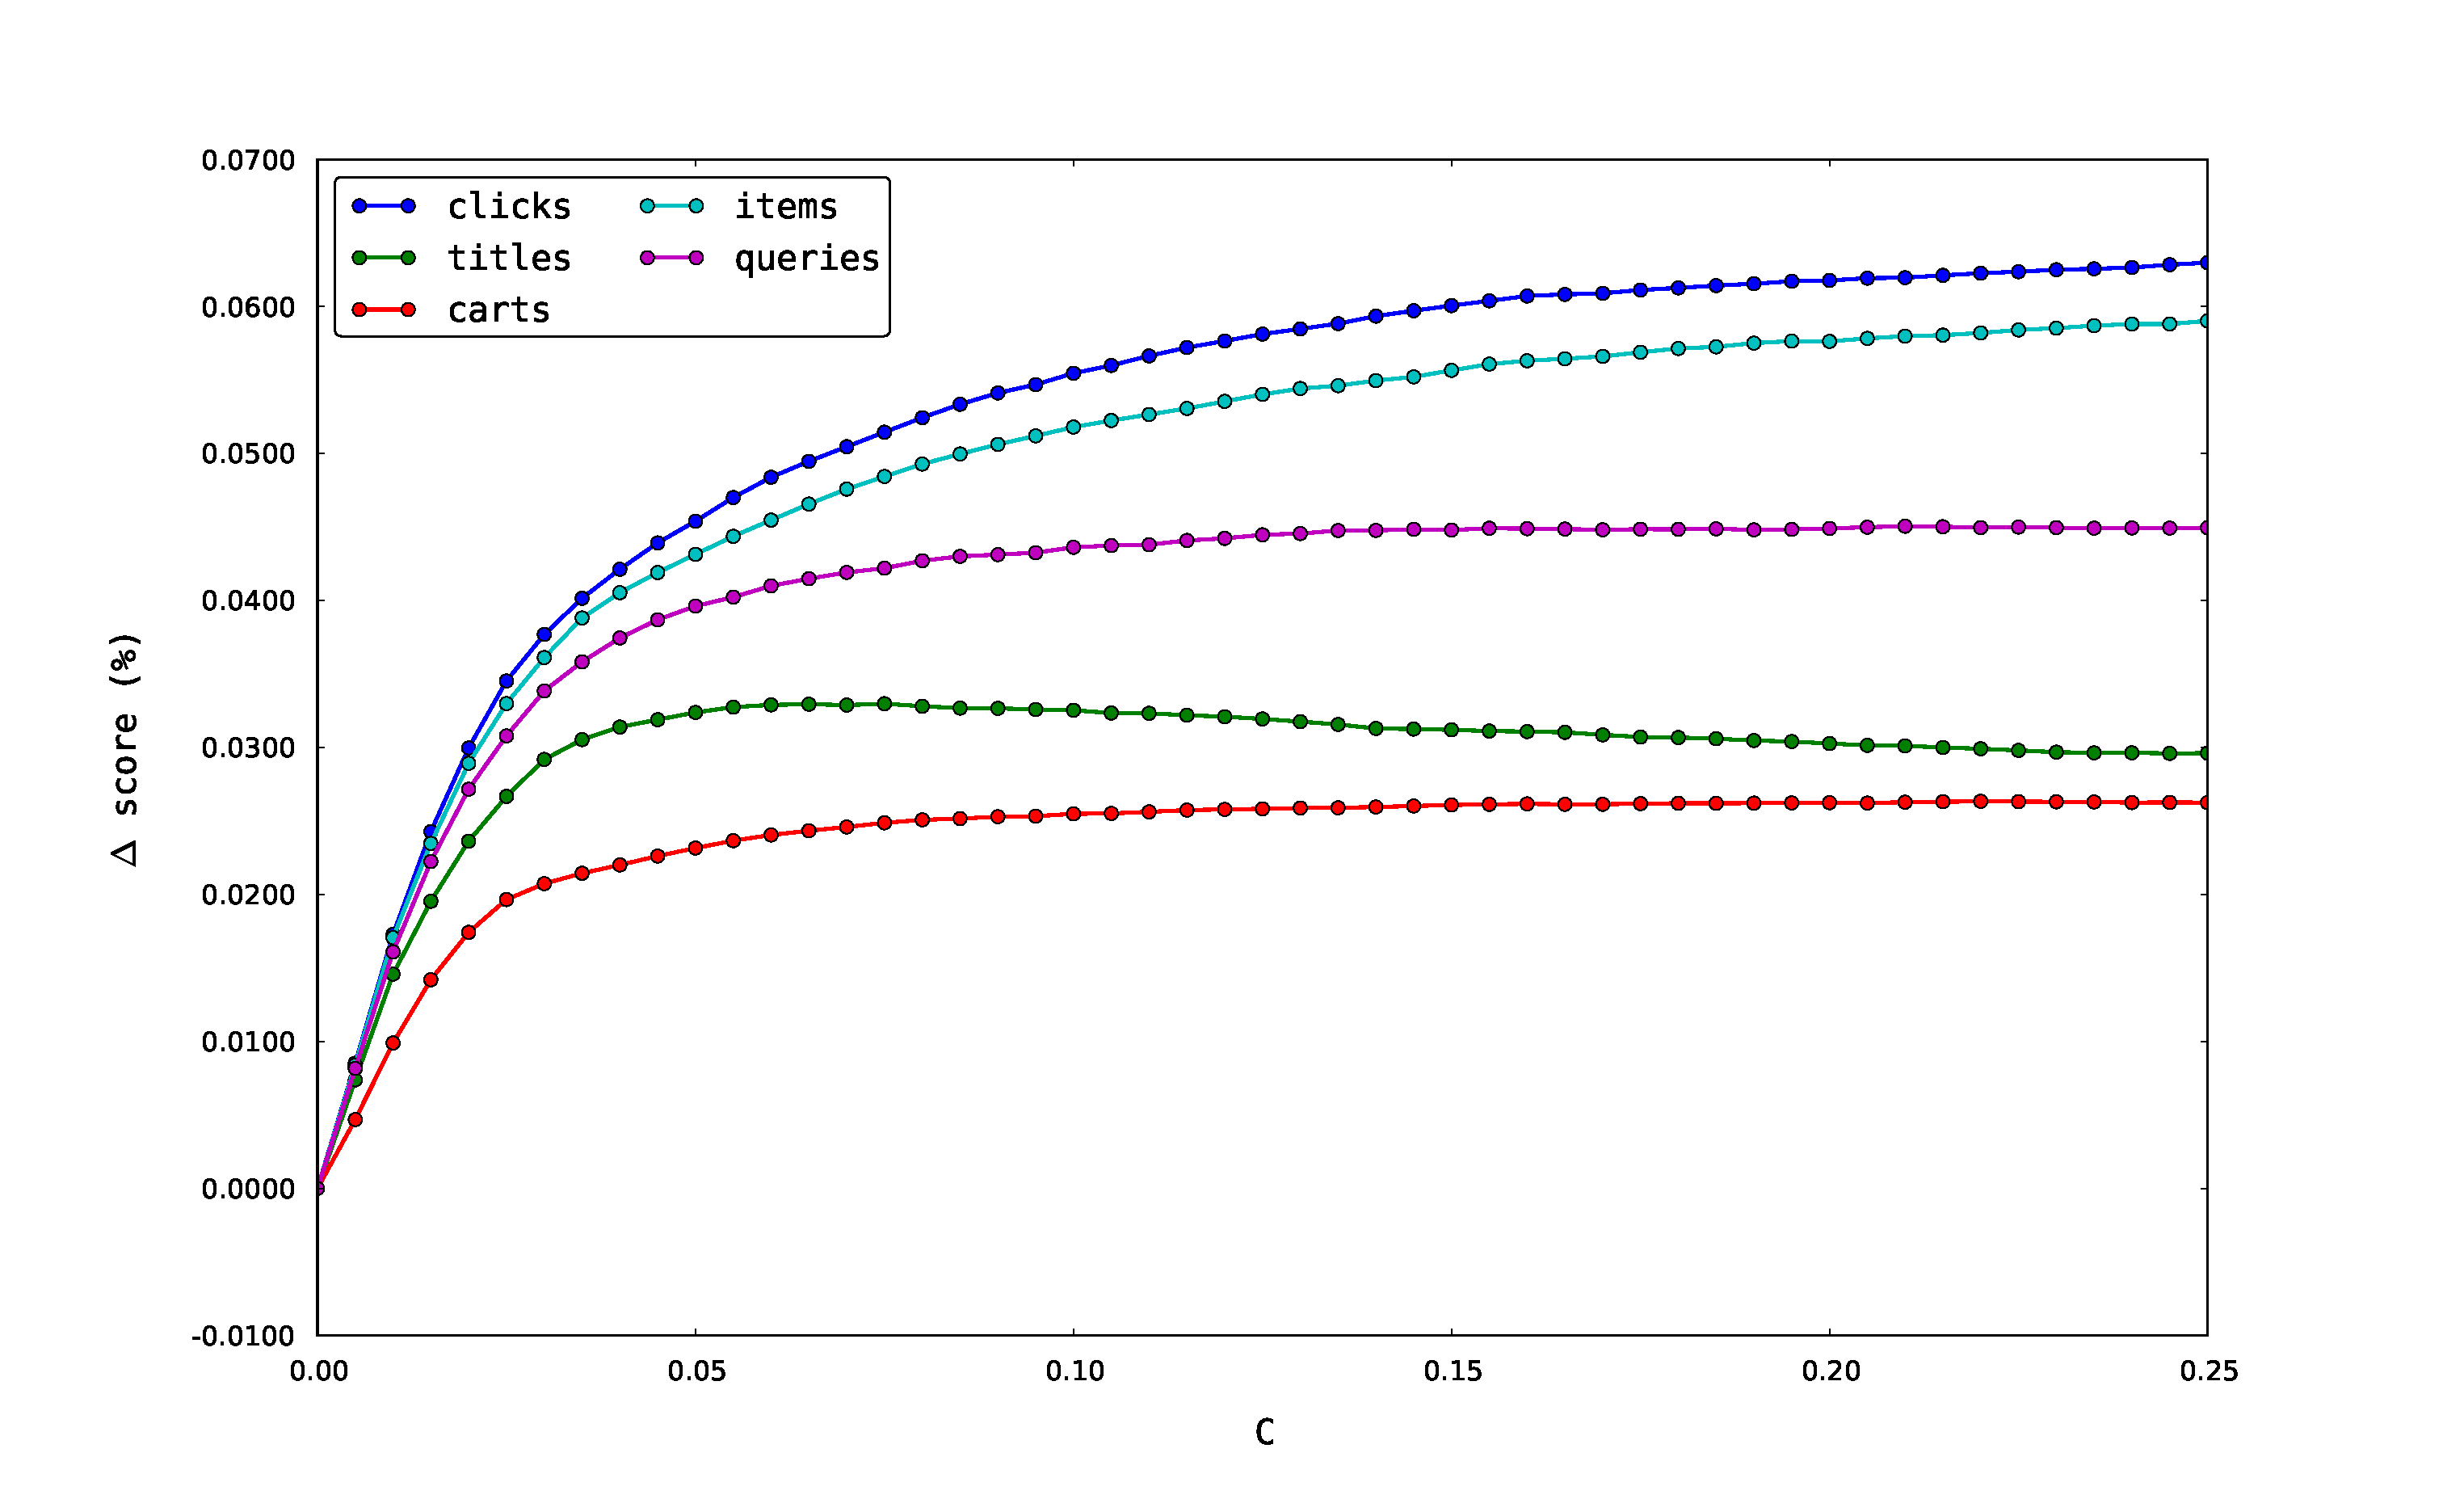
\includegraphics[width=\textwidth]{000050_0.48chunk.k100.i2.n100.percent_increase_position_score.0-0.25.eps}
\caption{\% increase of position score}
    \label{fig:percent_increase_of_position_score}
\end{figure}

\section{An Example}

To illustrate the efficacy of our technique, we present a real query example.
The only fictitious part of the example will be our shopper's name David.

David narrows his search space by selecting the category
``Grocery$\rightarrow$Beverages$\rightarrow$Water'' and made a query for
``water''. For the first few pages, Walmart presents David with a large
variety of different brands and sizes of packs of bottled water. These appear to
be reasonable results for any shopper making such a general query.
Unfortunately, packs of bottled water were not what David wanted to find. David
ended up clicking on and the 90th item presented by Walmart, ``Arrowhead
Mountain Spring Water, 3 l''. %picture?

It turns out that before making his query for ``water'', David had clicked on
the item ``Primo Ceramic Crock Water Cooler with Stand''. %picture?
Our technique recognized this previous click as a signal that David would be
interested in water products that are similar to his interest in the water
cooler stand. The reordered results generated by our technique 

was looking for 

\end{document}
